%
%Не забыть:
%--------------------------------------
%Вставить колонтитулы, поменять название на титульнике



%--------------------------------------

\documentclass[a4paper, 12pt]{article} 

%--------------------------------------
%Russian-specific packages
%--------------------------------------
%\usepackage[warn]{mathtext}
\usepackage[T2A]{fontenc}
\usepackage[utf8]{inputenc}
\usepackage[english,russian]{babel}
\usepackage[intlimits]{amsmath}
\usepackage{esint}
%--------------------------------------
%Hyphenation rules
%--------------------------------------
\usepackage{hyphenat}
\hyphenation{ма-те-ма-ти-ка вос-ста-нав-ли-вать}
%--------------------------------------
%Packages
%--------------------------------------
\usepackage{amsmath}
\usepackage{amssymb}
\usepackage{amsfonts}
\usepackage{amsthm}
\usepackage{latexsym}
\usepackage{mathtools}
\usepackage{etoolbox}%Булевые операторы
\usepackage{extsizes}%Выставление произвольного шрифта в \documentclass
\usepackage{geometry}%Разметка листа
\usepackage{indentfirst}
\usepackage{wrapfig}%Создание обтекаемых текстом объектов
\usepackage{fancyhdr}%Создание колонтитулов
\usepackage{setspace}%Настройка интерлиньяжа
\usepackage{lastpage}%Вывод номера последней страницы в документе, \lastpage
\usepackage{soul}%Изменение параметров начертания
\usepackage{hyperref}%Две строчки с настройкой гиперссылок внутри получаеммого
\usepackage[usenames,dvipsnames,svgnames,table,rgb]{xcolor}% pdf-документа
\usepackage{multicol}%Позволяет писать текст в несколько колонок
\usepackage{cite}%Работа с библиографией
\usepackage{subfigure}% Человеческая вставка нескольких картинок
\usepackage{tikz}%Рисование рисунков
\usepackage{float}% Возможность ставить H в положениях картинки
% Для картинок Моти
\usepackage{misccorr}
\usepackage{lscape}
\usepackage{cmap}



\usepackage{graphicx,xcolor}
\graphicspath{{Pictures/}}
\DeclareGraphicsExtensions{.pdf,.png,.jpg}

%----------------------------------------
%Список окружений
%----------------------------------------
\newenvironment {theor}[2]
{\smallskip \par \textbf{#1.} \textit{#2}  \par $\blacktriangleleft$}
{\flushright{$\blacktriangleright$} \medskip \par} %лемма/теорема с доказательством
\newenvironment {proofn}
{\par $\blacktriangleleft$}
{$\blacktriangleright$ \par} %доказательство
%----------------------------------------
%Список команд
%----------------------------------------
\newcommand{\grad}
{\mathop{\mathrm{grad}}\nolimits\,} %градиент

\newcommand{\diver}
{\mathop{\mathrm{div}}\nolimits\,} %дивергенция

\newcommand{\rot}
{\ensuremath{\mathrm{rot}}\,}

\newcommand{\Def}[1]
{\underline{\textbf{#1}}} %определение

\newcommand{\RN}[1]
{\MakeUppercase{\romannumeral #1}} %римские цифры

\newcommand {\theornp}[2]
{\textbf{#1.} \textit{ #2} \par} %Написание леммы/теоремы без доказательства

\newcommand{\qrq}
{\ensuremath{\quad \Rightarrow \quad}} %Человеческий знак следствия

\newcommand{\const}{\text{const}} % Написание const в формулах

\newcommand{\qlrq}
{\ensuremath{\quad \Leftrightarrow \quad}} %Человеческий знак равносильности

\renewcommand{\phi}{\varphi} %Нормальный знак фи

\newcommand{\me}
{\ensuremath{\mathbb{E}}}

\newcommand{\md}
{\ensuremath{\mathbb{D}}}



%\renewcommand{\vec}{\overline}




%----------------------------------------
%Разметка листа
%----------------------------------------
\geometry{top = 3cm}
\geometry{bottom = 2cm}
\geometry{left = 1.5cm}
\geometry{right = 1.5cm}
%----------------------------------------
%Колонтитулы
%----------------------------------------
\pagestyle{fancy}%Создание колонтитулов
\fancyhead{}
%\fancyfoot{}
\fancyhead[R]{\textsc{Экзамен. Оптика}}%Вставить колонтитул сюда
%----------------------------------------
%Интерлиньяж (расстояния между строчками)
%----------------------------------------
%\onehalfspacing -- интерлиньяж 1.5
%\doublespacing -- интерлиньяж 2
%----------------------------------------
%Настройка гиперссылок
%----------------------------------------
\hypersetup{				% Гиперссылки
	unicode=true,           % русские буквы в раздела PDF
	pdftitle={Заголовок},   % Заголовок
	pdfauthor={Автор},      % Автор
	pdfsubject={Тема},      % Тема
	pdfcreator={Создатель}, % Создатель
	pdfproducer={Производитель}, % Производитель
	pdfkeywords={keyword1} {key2} {key3}, % Ключевые слова
	colorlinks=true,       	% false: ссылки в рамках; true: цветные ссылки
	linkcolor=blue,          % внутренние ссылки
	citecolor=blue,        % на библиографию
	filecolor=magenta,      % на файлы
	urlcolor=cyan           % на URL
}
%----------------------------------------
%Работа с библиографией (как бич)
%----------------------------------------
\renewcommand{\refname}{Список литературы}%Изменение названия списка литературы для article
%\renewcommand{\bibname}{Список литературы}%Изменение названия списка литературы для book и report
%----------------------------------------
\begin{document}
	\begin{titlepage}
		\begin{center}
			$$$$
			$$$$
			$$$$
			$$$$
			{\Large{НАЦИОНАЛЬНЫЙ ИССЛЕДОВАТЕЛЬСКИЙ УНИВЕРСИТЕТ}}\\
			\vspace{0.1cm}
			{\Large{ВЫСШАЯ ШКОЛА ЭКОНОМИКИ}}\\
			\vspace{0.25cm}
			{\large{Факультет физики}}\\
			\vspace{5.5cm}
			{\Huge\textbf{{Экзамен}}}\\%Общее название
			\vspace{1cm}
			{\LARGE{<<Оптика>>}}\\%Точное название
			\vspace{2cm}
			\vfill
			
\includegraphics[width = 0.2\textwidth]{HSElogo}\\
			\vfill
			Москва\\
			2020
		\end{center}
	\end{titlepage}
	
	\tableofcontents
	
	\newpage
	
	\section{Световой луч. Распространение световых лучей. Оптическая длина пути. Принцип Ферма, понятие таутохронима в оптике. Законы отражения и преломления света.}

\textbf{Световым лучом} мы будем называть некоторый конечный, но очень узкий пучок, который может существовать изолированно от других лучей.

Согласно \textbf{закону прямолинейного распространения света} световые лучи в прозрачной \textit{однородной} среде распространяются прямолинейно. Согласно \textbf{закону о независимости световых пучков} распространение каждого светового луча не зависит от того, есть ли в среде иные световые лучи, или нет. Это разумеется, не совсем корректно: тогда бы не было явления интерференции, однако в рамках геометрической оптики мы этим явлением пренебрежем.

\textbf{Оптической длиной пути} $\Delta$ между двумя точками мы назовем расстояние, на которое свет распространился бы в вакууме за время прохождения расстояния между этими двумя точками. Как известно, скорость света в вакууме есть максимальная достижимая скорость и является константой $c$, а скорость света в веществе равна:

\begin{equation}
v = \frac{c}{n}
\label{eq:n_introduct}
\end{equation}

где $n$ --- абсолютный показатель преломления среды, который и вводится, как отношение скорости света в вакууме к скорости света в этой среде.

Тогда на основании формулы (\ref{eq:n_introduct}) можем записать:

\begin{equation*}
\Delta = n l
\end{equation*} 

где $l$ --- расстояние между точками, $n$ --- абсолютный показатель преломления среды.

Указанная формула имеет обобщение на случай, когда показатель среды может зависеть от координаты, тогда:

\begin{equation}
\Delta = \int\limits_a^b n dl
\label{eq:delta_introduct}
\end{equation} 

\theornp{Принцип Ферма}{Луч движется из начальной точки в конечную по траектории, которая обеспечивает минимальную оптическую длину пути. Является \textbf{постулатом}.} 

Из принципа Ферма в случае однородной среды логичным образом вытекает закон прямолинейного распространения света, упомянутый ранее.

% В оптике походу нет понятия таутохронима, ой

\theornp{Закон отражения света}{Луч падающий, луч отраженный и перпендикуляр, восстановленный из точки падения, лежат в одной полуплоскости. Угол падения равен углу отражения.}

\begin{theor}{Закон преломления света}{Луч падающий, луч преломленный и перпендикуляр, восстановленный в точке преломления, лежат в одной плоскости. Угол падения и угол преломления связаны следующим соотношением: $n_{1} \sin \alpha = n_{2} \sin \gamma$, где $n_1$ --- абсолютный показатель преломления среды, из которой луч приходит, $n_2$ --- среды, в которую луч преломляется, $\alpha$ --- угол падения, $\gamma$ --- угол преломления.}
	Пусть глаз наблюдателя находится на высоте H над поверхностью некоего водоема, а точечный источник --- на глубине $h$ в этом водоеме на расстоянии $S$ от места, где стоит наблюдатель (вдоль поверхности воды). Показатель преломления воздуха примем равным $n_{\text{возд}} = 1$, а показатель преломления воды --- $n$, известный нам.
	
	Пусть проекция отреза $BS$ на поверхность воды равна $x$. В таком случае:
	
	\begin{align*}
	BS&=\sqrt{h^{2}+x^{2}},\\
	MB&=\sqrt{H^{2}+(L-x)^{2}} \\ 
	t=\frac{SB}{v}+\frac{MB}{c}&=\left(n_{1}\sqrt{h^{2}+x^{2}}+\sqrt{H^{2}+(L-x)^{2}}\right) / c
	\end{align*}
	
	Согласно принципу наименьшего времени, полученное нами последнее выражение должно оказаться минимальным, другими словами $\dfrac{dt}{dx} = 0$ или:
	
	\begin{equation*}
	n_{1} \frac{x}{\sqrt{h^{2}+x^{2}}}-\frac{L-x}{\sqrt{H^{2}+(L-x)^{2}}}=0
	\end{equation*}
	
	\begin{figure}[H]
		\centering
		\includegraphics*[width=0.5\textwidth]{Snellius}
	\end{figure}
	
	В то же время из рисунка мы однозначно можем утверждать:
	
	\begin{align*}
	\sin \alpha &= \frac{x}{\sqrt{h^{2}+x^{2}}}\\
	\sin \gamma &= \frac{L-x}{\sqrt{H^{2}+(L-x)^{2}}}
	\end{align*}
	
	
	
	Отсюда напрямую следует факт:
	
	\begin{equation*}
	\boxed{n\sin\alpha = \sin\gamma}
	\end{equation*}
	
\end{theor}
	
	\newpage
	
	123
	
	\newpage
	
	123
	
	\newpage
	
	123
	
	\newpage
	
	123
	
	\newpage
	
	123
	
	\newpage
	
	
	\section{Плоская монохроматическая волна. Представление монохроматических волн в
		комплексном виде. Сферическая и цилиндрическая волны. Стоячие электромагнитные
		волны. Опыты Винера.}
	(ЛЛ2 \S 46 и дальше)\\
	\subsection*{Плоские волны}
	Стартуем с обычного волнового уравнения:
	\begin{align*}
	\Delta A - \dfrac{1}{c^2} \dfrac{\partial^2}{\partial t^2}A = 0
	\end{align*}
	Где A - это вектор потенциал, так же помним что такое уравнение было полученно при калибровке $\diver A = 0$. Понятно, что для напряженности электрического и магнитного поля верны такие же уравнения. Хотим изучать плоские волны, это значит, что вектор потенциал может зависить только от одной координаты. Для определенности это x. Тогда уравнение выглядит так:
	\begin{align}
	\dfrac{\partial^2}{\partial x^2}\vec{A} - \dfrac{1}{c^2} \dfrac{\partial^2}{\partial t^2}\vec{A} = 0
	\label{7_1eq}
	\end{align}
	Калибровочное условие превращается в $ \dfrac{\partial}{\partial x}A_x = 0$, значит $\dfrac{\partial^2}{\partial t^2}A_x  = 0$. Отсюда логично заключить, что x компонента потенциала либо линейна по времени, либо ее нет. Первое означало бы наличие постоянного электрического поля, что никакого отношения к волнам не имеет. Значит $A_x = 0$. То есть вектор потенциал всегда лежит в плоскости перпендикулярной направлению движения. Для любого, кто читал конспект по матфизу очевидно, что решением уравнения (\ref{7_1eq}) будет любая функция $\vec{A}(t - \dfrac{x}{c})$ понятно что волна еще может лететь влево, но опустим это, там все то же самое. Из этого решения следует, что 
	\begin{align}
	\dfrac{\partial A}{\partial t} = -\dfrac{1}{c} \dfrac{\partial A}{\partial x}
	\label{7_2eq}
	\end{align}
	Пока запомним это. Теперь вычислим E и H, помня, что вектор потенциал зависит только от x
	\begin{align*}
	\vec{H} = - \vec{e}_y \partial_x A_z + \vec{e}_z \partial_x A_y\\
	\vec{E} = -\dfrac{1}{c} \vec{e}_y\dfrac{\partial A_y}{\partial x} -\dfrac{1}{c} \vec{e}_z \dfrac{\partial A_z}{\partial x}\\
	\vec{E}\vec{H} = -\dfrac{1}{c^2} \partial_x A_y \partial_x A_z +\dfrac{1}{c^2} \partial_x A_y \partial_x A_z = 0
	\end{align*}
	Здесь мы воспользовались формулой (\ref{7_2eq}). Теперь мы знаем, что в любой плоской волне электрическое поле перпендикулярно электрическому. И лежат они в одной плоскости, перпендикулярной направлению распространения волны. Кстати, по модулю они равны, что видно из уравнений выше. Так что можно смело написать:
	\begin{align*}
	S = \dfrac{c}{4\pi} [\vec{E} \vec{H}] = \dfrac{c E^2}{4\pi}\vec{n} = \dfrac{cH^2}{4\pi}\vec{n}
	\end{align*}
	Где вектор n единичный в направлении распространения. \\
	Что такое монохроматическая волна? Это когда $\dfrac{1}{c^2} \dfrac{\partial^2}{\partial t^2}\vec{A} =- \dfrac{\omega^2}{c^2} \vec{A}$, фактически фурье компонента. Если подставить это в уравнение (\ref{7_1eq}), то получим обычное уравнение на гармонический осциллятор для координаты. Значит итоговое решение будет:
	\begin{align*}
	\vec{A} = 	Re\{ \vec{A}_0 e^{-i \omega (t - x/c)}\}
	\end{align*}
	Действительную часть мы взяли потому, что поля не бывают комплексными. А вот $A_0$ бывает. Поэтому правильным выбором $A_0$ волну можно сделать любой комбинацией синусов и косинусов которая нужна. Если взять от этой штуки частную производную по времени, что получить поле не сложно:
	\begin{align*}
	\vec{E} = 	Re\{ \vec{E}_0 e^{-i \omega (t - x/c)}\}
	\end{align*}
	Введя вектор $\vec{k} = \dfrac{\omega}{c} \vec{n}$ можно отвязаться от координат и просто написать
	\begin{align*}
	\vec{E} = 	Re\{ \vec{E}_0 e^{i (kr - \omega t)}\}
	\end{align*}
	Обычно взятие действительной части опускают. Так пока мы совершаем линейные операции с полями нам это не важною.  \\
	\subsection*{Сферические и цилиндрические волны}
	Для простоты рассмотрим только монохроматические. Сферические волны это когда зависимость есть только от расстояния до начала координат. Вспоминая как вылгядит оператор лапласа в сферике (например в вики) и быстро решая уравнение получаем (Re опустил):
	\begin{align*}
	A = A_0 \dfrac{e^{i (kr - \omega t)}}{r}
	\end{align*}
	Теперь пишем дифур на цилиндрические волны. \textbf{Здесь r - расстояние до оси}
	\begin{align*}
	&\dfrac{1}{r} \partial_r (r \partial_r f) + k^2 f = 0\\
	& x = r k\\
	&f'' + \dfrac{1}{x} f' + f = 0
	\end{align*} 
	А это уравнение на функцию Бесселя. Конечно есть еще функция Неймана, но нам надо чтобы в нуле значение было конечным, а функция Неймана этого не дает. Итого решениe пропорцианально такой штуке: $J_0(k r) e^{-i\omega t}$ на больших временах можно написать асиптотику: 
	\begin{align*}
	A_0 \dfrac{e^{i (kr - \omega t - \pi/4)}}{\sqrt{r}}
	\end{align*}
	\subsection*{Стоячие волны и опыт Винера}
	Если есть две одинаковые волны $e^{i (kr - \omega t)} \quad e^{i (-kr - \omega t)}$, идущие в разных направлениях (например после отражения), то их можно сложить и получить $2\cos \omega t \cos k r$\\
	Но физически мы можем заметить только квадрат амплитуды. Ну тут видно, что после усреднения по времени мы будем наблюдать серию кучностей на расстоянии по $\lambda/2$ друг от друга. Проблема в их наблюдении это малая длина волны. Вот что придумал Винер.\\
	Берем фоточувствительную пластинку и ставим ее под малым углом к зеркалу. Освещаем зеркало монохроматическим светом на наблюдаем тучности непосредственно
	\begin{figure}[H]
		\centering
		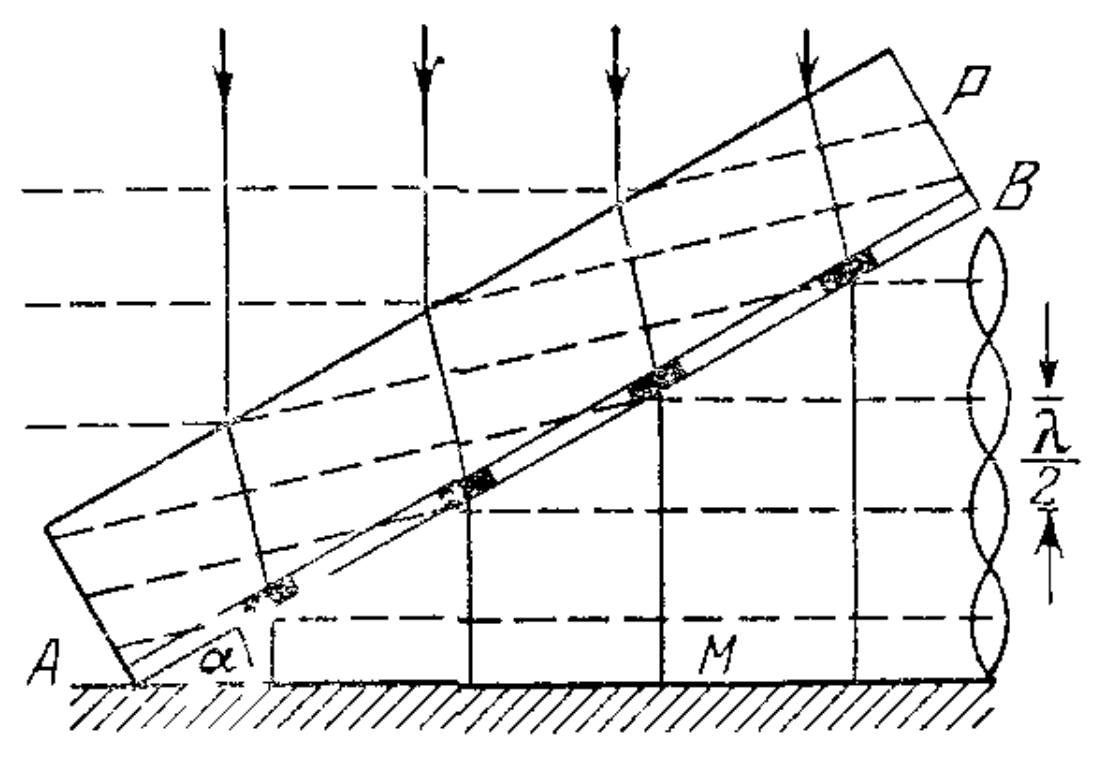
\includegraphics[scale = 0.3]{7_1}
	\end{figure}
	Расстояние между ними по прямой будет $\dfrac{\lambda}{2 \sin \alpha}$, то есть зная синус наклона можно узнать и длину волны.  
	
	\newpage
	
	123
	
	\newpage
	
	123
	
	\newpage
	
	123
	
	\newpage
	
	123
	
	\newpage
	
	123
	
	\newpage
	
	123
	
	\newpage
	
	123
	
	\newpage
	
	123
	
	\newpage
	
	123
	
	\newpage
	
	
	\section{Понятие о когерентности. Частично когерентный свет. Основные интерференционные
		схемы. Интерференция плоских волн, пространственный период полос.}
	Монохроматических волн не бывает в природе. В реальности волны часто излучаются модулированными как по амплитуде, так и по частоте. Такие называют квазимонохроматическими. 
	\begin{align*}
	a(t) \cos (\omega t + b(t))
	\end{align*}
	\textbf{когерентными наз ывают две волны, если у них постоянная разность фаз}\\
	Так две монохроматические волны когерентны, если у них одинаковая частота.\\
	Если есть какая-то маленькая разница в частотах $\Delta \omega$ то говорят о времени когерентности $t \Delta \omega \sim \pi$. Предполагаю малость $\Delta \omega$ получаем $t \sim \dfrac{\lambda^2}{2c \Delta \lambda}$ отсюда получается то, что называют длинной когерентности $l \sim \dfrac{\lambda^2}{2\Delta \lambda}$\\
	Пусть у нас есть две плоские волны. 
	\begin{align*}
	A_1 = a_1 \cos \mathbf{k_1 r} - \omega t + \phi_1\\
		A_2 = a_2 \cos \mathbf{k_2 r} - \omega t + \phi_2
	\end{align*}
	Тогда не сложно их сложить и получить распределение интенсивности
	\begin{align*}
	I = I_1 + I_2 + 2\sqrt{I_1 I_2} \cos( \mathbf{(k_1 - k_2)r} + \phi_1 - \phi_2 )
	\end{align*}
	Ага, теперь мы знаем, что интенсивность постоянна в плоскостях перпендикулярных $\mathbf{k_1 - k_2}$ \\
	Расстояние между плоскостями максимумов будет $\dfrac{2\pi}{|\mathbf{k_1 - k_2}|}$. Для равных по модулю векторов $\dfrac{\lambda}{2 \sin \alpha/2}$ где альфа это угол между векторами\\
	\subsection{Основные схемы}
	\textbf{Схема Юнга.} 
	\begin{figure}[h]
		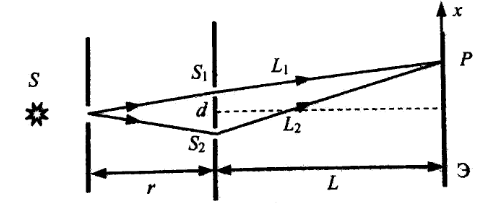
\includegraphics[scale = 0.7]{17_1}
	\end{figure}
	Ширина полос и расстояние между ними равно $\dfrac{\lambda L}{d}$\\ 
	\textbf{Тонкий клин.} В приближении малых углов падения и малости угла альфа просто поворачивает входной луч на $(n-1)\alpha$\newpage
	\begin{figure}[h]
		\centering
		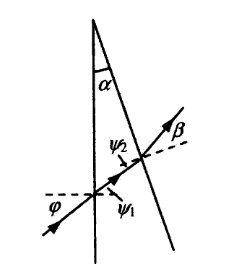
\includegraphics[scale = 0.7]{17_2}
	\end{figure}
	\textbf{Бипризма Френеля} Две призмы из прошлого пункта. В итоге получаем, что эффективно один источник расслаивается на два. Расстояние между ними $2a(n-1)\alpha$, и теперь задача свелась просто к опыту Юнга \\
	\begin{figure}[H]
		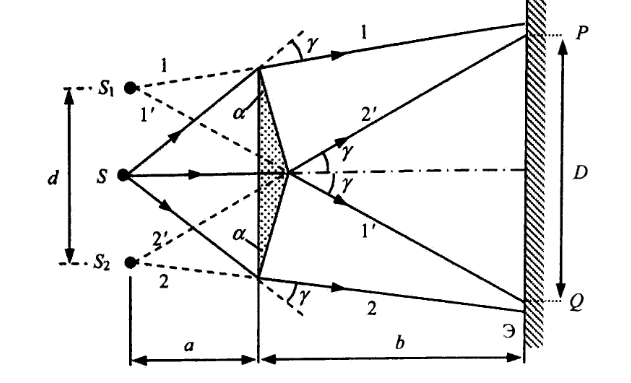
\includegraphics[scale = 0.5]{17_3}
	\end{figure}

	
	\newpage
	
	123
	
	\newpage
	
	123
	
	\newpage
	
	123
	
	\newpage
	
	123
	
	\newpage
	
	
	\section{Пространственная когерентность. Радиус пространственной когерентности,
		зависимость радиуса пространственной когерентности от угловых размеров
		источника света.}
	Будем рассматривать пространственную когерентность на примере опыта Юнга. \\
	 \begin{figure}[H]
	 	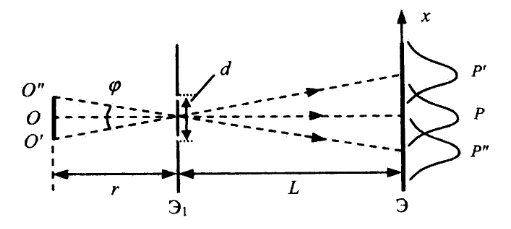
\includegraphics[scale = 0.6]{22_1}
	 \end{figure}
	 Пусть источник света имеет какие-то линейные размеры. Тогда каждая точка источника создает свою интерференционную картину, которые наслаиваются друг на друга. Как известно период полос $\dfrac{\lambda L}{d}$ а сдвиг за счет неточечности будет $\phi L$ итого получаем условие $b < \dfrac{\lambda}{\phi}$ это и называют радиусом когерентности. $ \rho = \dfrac{\lambda}{\phi}$

	
	\newpage
	
	123
	
	\newpage
	
	123
	
	\newpage
	
	123
	
	\newpage
	
	123
	
	\newpage
	
	
	\section{Многолучевая интерференция. Интерферометр Фабри-Перо. Формула Эйри.
		Пластинка Люммера-Герке. Интерференционные фильтры и зеркала. Просветление
		оптики.}
	\begin{figure}[h]
		\centering
		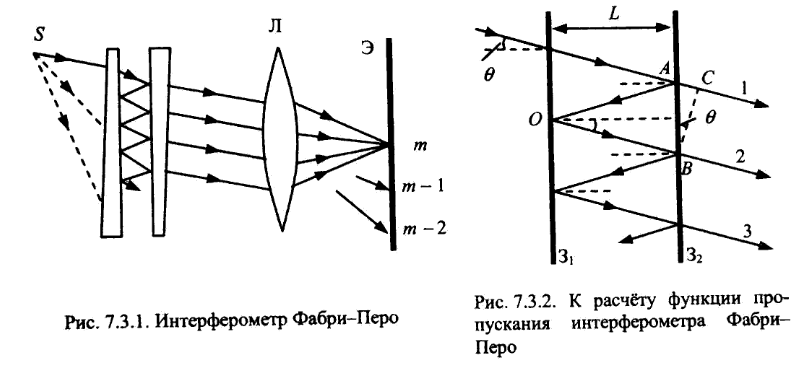
\includegraphics[scale = 0.7]{27_1}
	\end{figure}
	Интерферометр Фабри-Перо это два почти идеальных зеркала, которые отражают $\sim 99\%$ а оставшееся пропускают. Луч, попадая в нее испытывает многократные отражения. Обычно после интерферометра ставят линзу, что бы собрать параллельный пучек в точку.  Итак, пусть луч падает под углом $\theta$ на интерферометр. Надо думать, что он маленький, иначе не множественных отражений просто не будет. За один проход луч неберает фазу $\Delta = AOC - AB = \dfrac{2L}{\cos \theta} - 2L \tan \theta \sin \theta = 2L \cos \theta$ получается условие на максимумы будет иметь вид $2L \cos \theta = \lambda m$ \
	Пусть мы отражаемся много раз. Пусть на интерферометр падает луч с амплитудой $A$ и фазой ноль, тогда тот луч, который прошел ни разу не отразившись будет иметь $Ad^2$ тот который 2 раза отразился перед выходом $Ad^2 r^2 e^{i\delta}$  и так далее. Если угол тета мал, то отражений будет очень много, а $r^2 <1$ то просуммировав ряд получим:
	 \begin{align*}
	 A_{конечная} = Ad^2 \dfrac{1}{1 - r^2 e^{i\delta}}\\
	 \delta = 2L k\cos \theta\\
	 D = \dfrac{(1 - r^2)^2}{1 - 2r^2 \cos \delta + r^4}
	 \end{align*}
	 D это энергетический коэффициент пропускания. Так же это называется формулой Эйри, если судить по презентациям лектора.\\
	 \begin{figure}[t!]
	 	\centering
	 	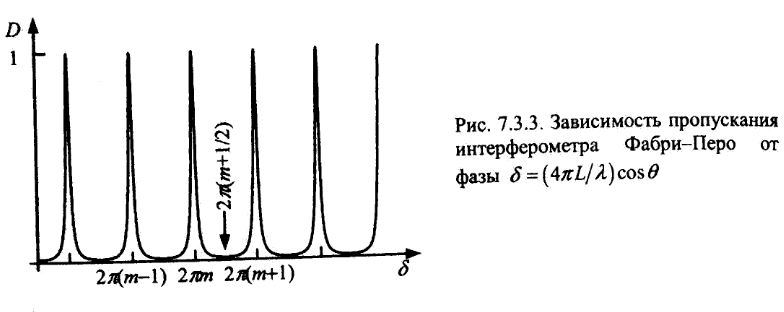
\includegraphics[scale = 0.5]{27_2}
	 \end{figure}
	 	Посмотрим на пластинку Люммера-Герке.
		\begin{figure}[h]
			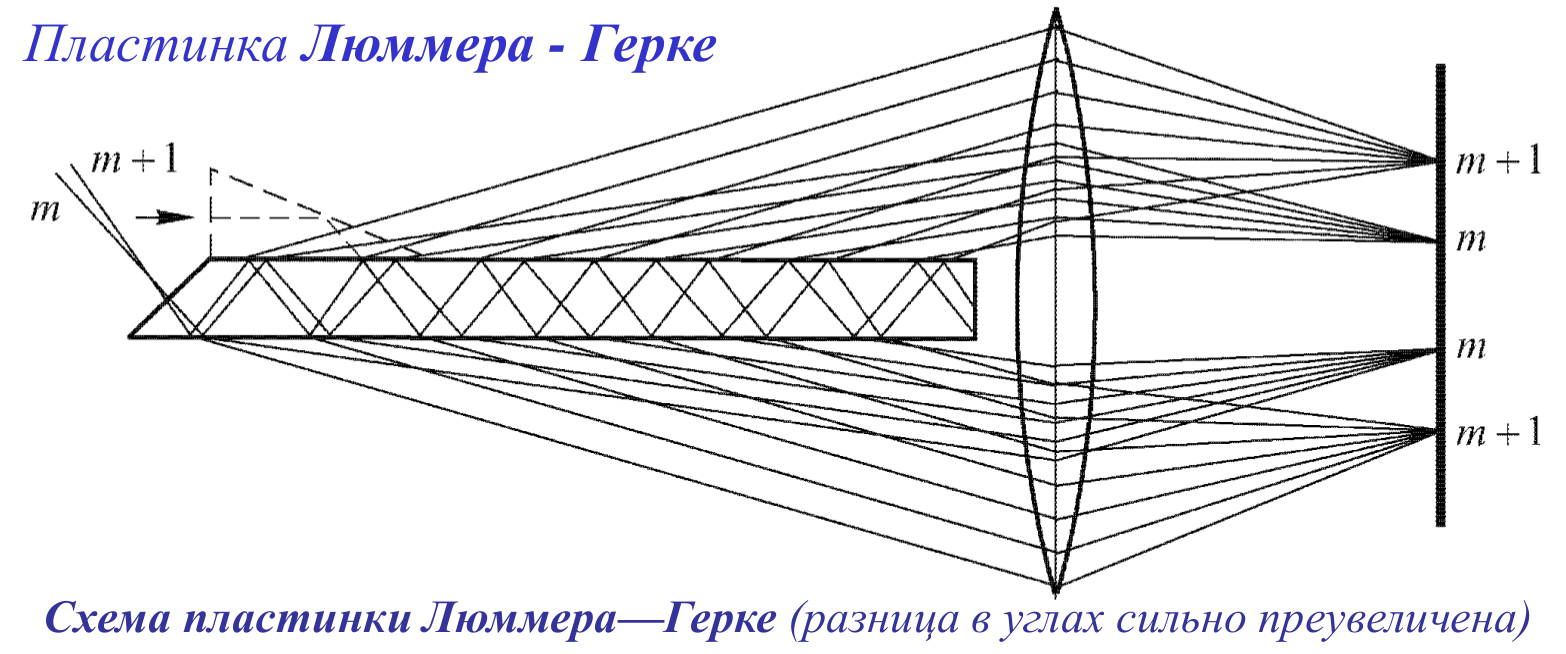
\includegraphics[scale = 0.3]{27_3}
		\end{figure}
		Что-то очень похожее на Фабри-Перо. Очевидно, что максимумы достигаются при условии $2d n \cos \theta = \lambda m$ где d толщина, а n- оптическая плотность \newpage
		\textbf{Просветление оптики}
		Допустим мы недовольны коэффициентом отражения стекла. Тогда мы можем нанести тонкий слой чего-нибудь на поверхность, главное чтобы это что-нибудь имело n меньше, чем у нашего стекла. При условии $\delta = \dfrac{2\pi}{\lambda} 2nh = (2m + 1)$ отраженная от первого края волна и отраженная от второго погасят друг друга и коэффициент прохождения увеличится.
		\begin{figure}[H]
			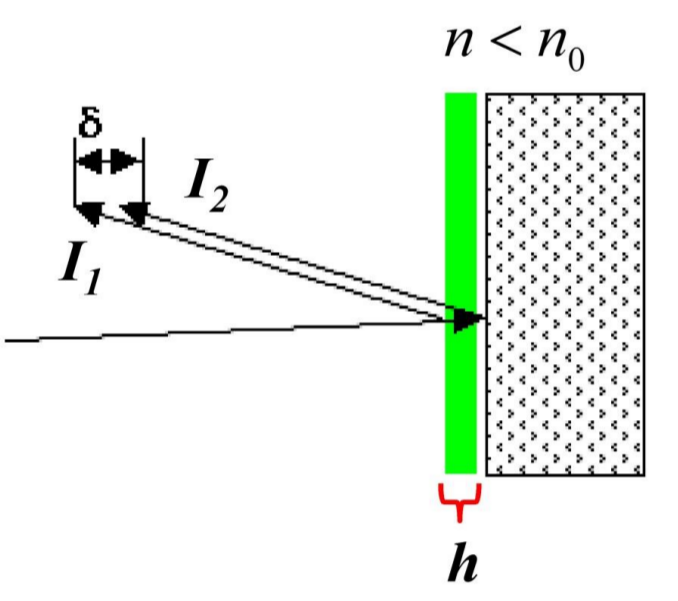
\includegraphics[scale = 0.3]{27_4}
		\end{figure}
	
	\newpage
	
	123
	
	\newpage
	
	123
	
	\newpage
	
	123
	
	\newpage
	
	123
	
	\newpage
	
	123
	
	\newpage
	
	123
	
	\newpage
	
	123
	
	\newpage
	
	123
	
	\newpage
	
	123
	
	\newpage
	
	123
	
	\newpage
	
	123
	
	\newpage
	
	123
	
	\newpage
	
	123
	
	\newpage
	
	123
	
	\newpage
	
	123
	
	\newpage
	
	123
	
	\newpage
	
	123
	
	\newpage
	
	123
	
	\newpage
	
	123
	
	\newpage
	
	123
	
	\newpage
	
	123
	
	\newpage
	
	123
	
	\newpage
	
	123
	
	
	
	
	
	
	
	
	
	
	
	
\end{document}